\section{Analysis}

\subsection{Data Exploration}

The demographic data for the general population of Germany contains 366 features, and to display it here, we have to transpose it. Below are the first 5 samples from the first 10 features (for all the features, please see table \ref{tab:AZDIAS} in the ANNEX section):

\subfile{./tables/azdias_short}

The feature names are not very explanatory, but fortunately for us along with the datasets, we have two other files:

\begin{itemize}
\item \emph{DIAS Information Levels - Attributes 2017.xlsx}: Describes each feature.
\item \emph{DIAS Attributes - Values 2017.xlsx}: Describes the type of each feature along with possible values along with values that represent missing or unknown information.
\end{itemize}

As we can see the dataset contains a lot of missing values (represented by NaN in table \ref{tab:AZDIAS_SHORT} and \ref{tab:AZDIAS}) and some of the values, like (-1, 0 or 9) also indicate missing or unknown information.

Based on the \emph{DIAS Attributes - Values 2017.xlsx} we've built a new dataset \emph{AZDIAS\_Feature\_Summary.csv} that contains a summary of properties for each demographics data column, as follows (for the full list please see table \ref{tab:FEAT_INFO} in the ANNEX section):

\subfile{./tables/feature_info_short}

We use this file to help us make cleaning decisions for the project. 

\paragraph{Missing Values} 
The third column (\emph{missing\_or\_unknown} of the feature attributes summary, documents the codes from the data dictionary that indicate missing or unknown data. Before converting data that matches a 'missing' or 'unknown' value code into a NaN value, we first have a look how much data takes on a 'missing' or 'unknown' code, and how much data is naturally missing, as a point of interest.

\paragraph{Select and Re-Encode Features}
Checking for missing data isn't the only way in which we can prepare a dataset for analysis. Since the unsupervised learning techniques we use only work on data that is encoded numerically, we need to make a few encoding changes or additional assumptions to be able to make progress. While almost all of the values in the dataset are encoded using numbers, not all of them represent numeric values.

\begin{itemize}
    \item For numeric and interval data, these features can be kept without changes.
    \item Most of the variables in the dataset are ordinal. While ordinal values may technically be non-linear in spacing, we make the simplifying assumption that the ordinal variables can be treated as being an interval in nature (that is, kept without any changes).
    \item Special handling may be necessary for the remaining two variable types: categorical, and 'mixed.'
\end{itemize}

\paragraph{Categorical Features}
For categorical features, we encode the levels as dummy variables. Depending on the number of categories, we can perform one of the following:
\begin{itemize}
    \item For binary (two-level) categorical features that take numeric values, we can keep them without needing to do anything.
    \item If there are binary variables that take on non-numeric values, we need to re-encode the values as numbers or create a dummy variable.
    \item For multi-level categorical features (three or more values), we can choose to encode the values using multiple dummy variables (e.g., via \emph{OneHotEncoder})
\end{itemize}

\paragraph{Mixed-Type Features}
There are a handful of features that are marked as "mixed" in the feature summary that require special treatment before we can include then in the analysis. There are two in particular that deserve attention:

\begin{itemize}
    \item \emph{PRAEGENDE\_JUGENDJAHRE} combines information on three dimensions: generation by decade, movement (mainstream vs. avantgarde), and nation (east vs. west). While there aren't enough levels to disentangle east from west, we create two new variables to capture the other two dimensions: an interval-type variable for the decade, and a binary variable for movement.
    \item \emph{CAMEO\_INTL\_2015} combines information on two axes: wealth and life stage. We break up the two-digit codes by their 'tens'-place and 'ones'-place digits into two new ordinal variables (which, for this project, is equivalent to just treating them as their raw numeric values).
\end{itemize}

\paragraph{Ordinal and Interval Features}
Nothing special here, we need to decide what to do with the missing values

\paragraph{Numerical Features}
Nothing special here, we need to decide what to do with the missing values and perhaps perform some scaling.

\subsection{Exploratory Visualization}

Figure \ref{fig:before_unknown}, obtained using the \emph{missingno} package shows the missing values of the provided data and figure \ref{fig:after_unknown} same information but after we replaced the unknown or missing value codes with NaN.

\begin{figure}[h]
  \centering
  \subfloat{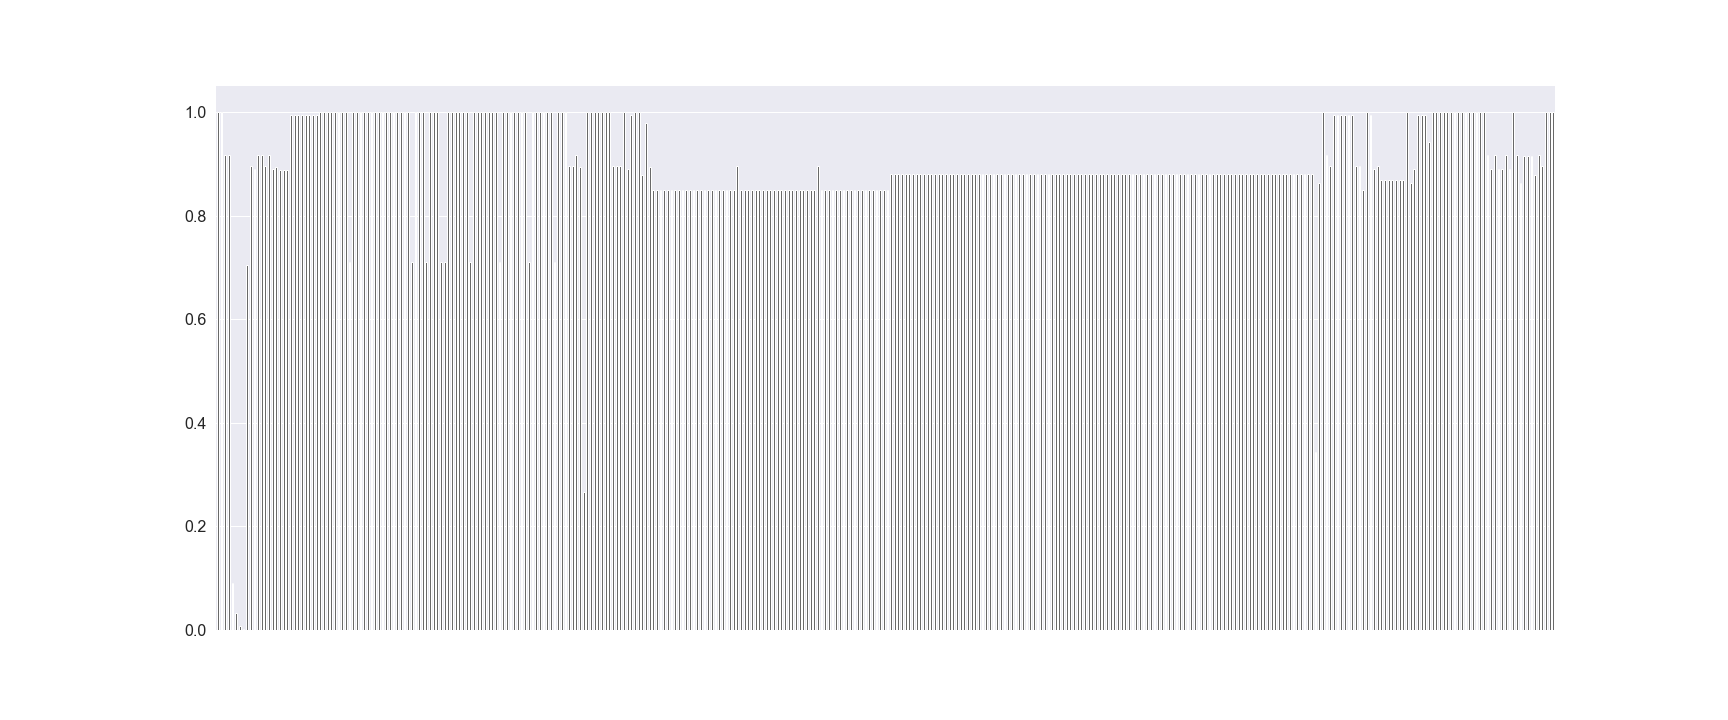
\includegraphics[width=0.5\textwidth]{images/before_unknown.png}\label{fig:before_unknown}}
  \hfill
  \subfloat{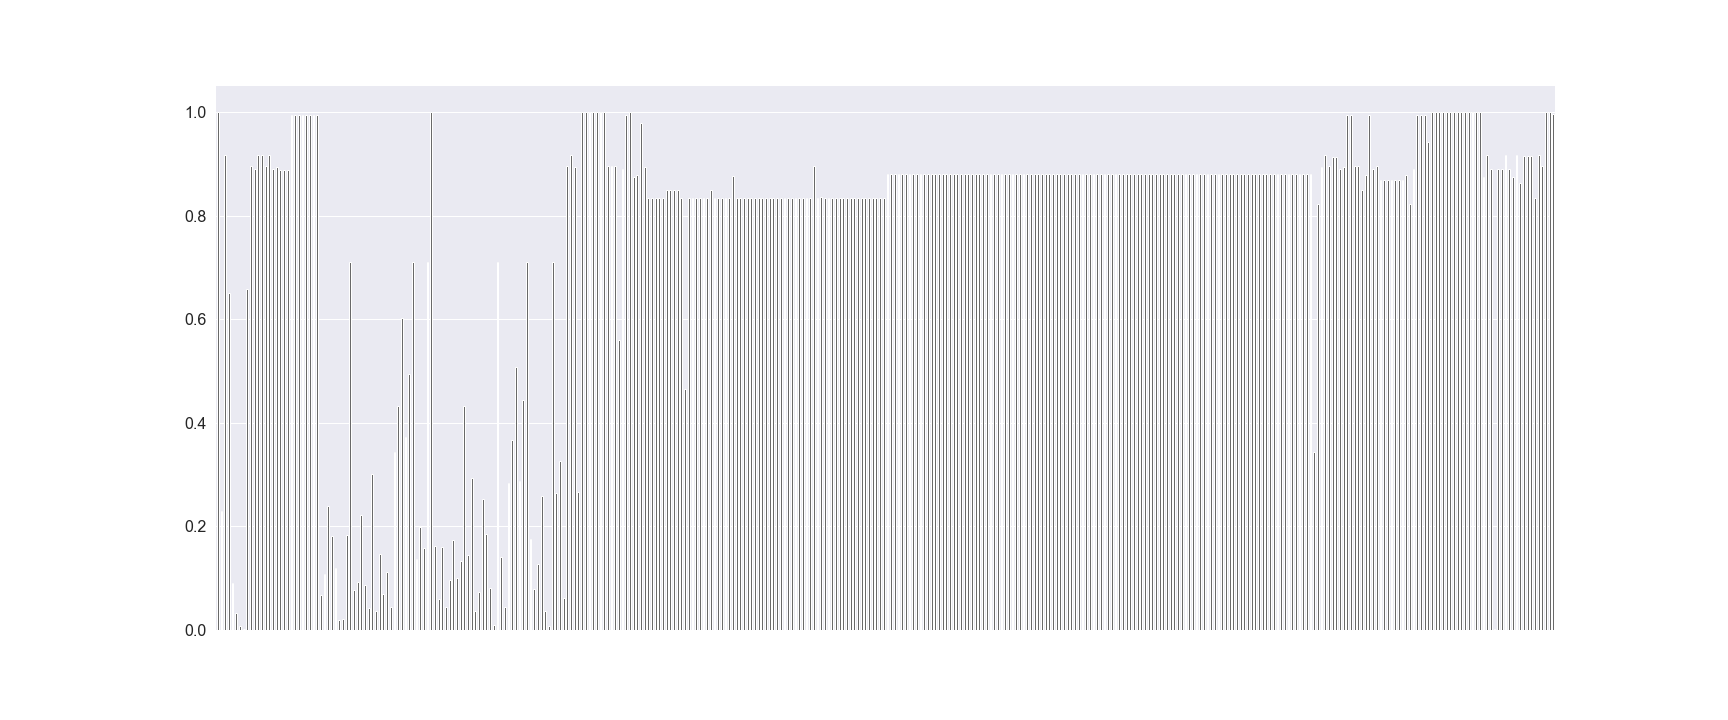
\includegraphics[width=0.5\textwidth]{images/after_unknown.png}\label{fig:after_unknown}}
  \caption{Missing values per column before and after replacing unknown value codes}
\end{figure}

In figure \ref{fig:column_nans} we have the distribution of missing value counts where we can see that that there are a few columns that are outliers in terms of the proportion of values that are missing. We also perform a similar assessment for the rows of the dataset to asses how much data is missing in each row (see figure \ref{fig:row_nans}). As with the columns, we see some groups of points that have a very different number of missing values.

\begin{figure}[h]
  \centering
  \subfloat[Distribution of missing value counts per column]{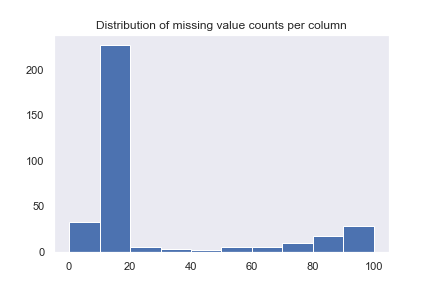
\includegraphics[width=0.5\textwidth]{images/column_nans.png}\label{fig:column_nans}}
  \hfill
  \subfloat[Distribution of missing value counts per rows]{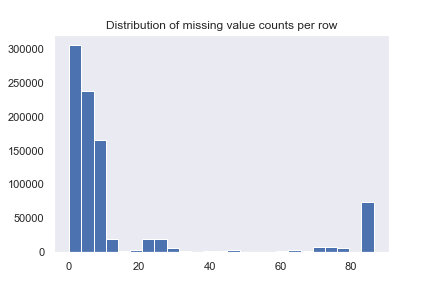
\includegraphics[width=0.5\textwidth]{images/row_nans.png}\label{fig:row_nans}}
  \caption{Distribution of missing value counts per column and row}
\end{figure}

\subsection{Algorithms and Techniques}

There are 2 parts of this project:

\paragraph{Unsupervised modeling}
The main bulk of our analysis is in this part of the project. Here, we use unsupervised learning techniques to describe the relationship between the demographics of the company's existing customers and the general population of Germany. By the end of this part, we should be able to describe parts of the general population that are more likely to be part of the mail-order company's primary customer base, and which parts of the general population are less so.

We first apply PCA (Principal Component Analysis) \cite{PCA} to reduce the dimensionality of the dataset \cite{jonathonshlens2005}. We decide on a number of components that explain at least 90\% of the variance in data. 

After PCA, we create KMeans\cite{KMeans} models with clusters from 2 to 15. Clustering is a method of unsupervised learning, where each data point or cluster is grouped into a subset or a cluster, which contains similar kind of data points. We decide on the best number of clusters to take based on the Elbow\cite{dtpham2004} method.

\paragraph{Supervised modeling}
To predict the probability of a person to reply to the mailing campaign, we create an XGBoostClassifier model which we use to predict this probability.

Before training the model, we decide on a resampling technique for the data, and after we start by searching the best hyperparameters for models using all available features by using a Bayesian search.

Once we have a list of optimized hyperparameters, we use them for training a model on the resampled data.
After training the model is used to predict on the TEST dataset.

\subsection{Benchmark}

Model evaluation is the process of objectively measuring how well machine learning models perform the specific tasks they were designed to do.

We use the AUC scores to benchmark the performance of the models. A model with the highest AUC is considered as the best performer. We train a LogisticRegression model with default parameters and use it to predict the probabilities for the train and test datasets. The obtained AUC score is our base score used for comparison.